\documentclass[twoside]{book}

% Packages required by doxygen
\usepackage{fixltx2e}
\usepackage{calc}
\usepackage{doxygen}
\usepackage[export]{adjustbox} % also loads graphicx
\usepackage{graphicx}
\usepackage[utf8]{inputenc}
\usepackage{makeidx}
\usepackage{multicol}
\usepackage{multirow}
\PassOptionsToPackage{warn}{textcomp}
\usepackage{textcomp}
\usepackage[nointegrals]{wasysym}
\usepackage[table]{xcolor}

% Font selection
\usepackage[T1]{fontenc}
\usepackage[scaled=.90]{helvet}
\usepackage{courier}
\usepackage{amssymb}
\usepackage{sectsty}
\renewcommand{\familydefault}{\sfdefault}
\allsectionsfont{%
  \fontseries{bc}\selectfont%
  \color{darkgray}%
}
\renewcommand{\DoxyLabelFont}{%
  \fontseries{bc}\selectfont%
  \color{darkgray}%
}
\newcommand{\+}{\discretionary{\mbox{\scriptsize$\hookleftarrow$}}{}{}}

% Page & text layout
\usepackage{geometry}
\geometry{%
  a4paper,%
  top=2.5cm,%
  bottom=2.5cm,%
  left=2.5cm,%
  right=2.5cm%
}
\tolerance=750
\hfuzz=15pt
\hbadness=750
\setlength{\emergencystretch}{15pt}
\setlength{\parindent}{0cm}
\setlength{\parskip}{3ex plus 2ex minus 2ex}
\makeatletter
\renewcommand{\paragraph}{%
  \@startsection{paragraph}{4}{0ex}{-1.0ex}{1.0ex}{%
    \normalfont\normalsize\bfseries\SS@parafont%
  }%
}
\renewcommand{\subparagraph}{%
  \@startsection{subparagraph}{5}{0ex}{-1.0ex}{1.0ex}{%
    \normalfont\normalsize\bfseries\SS@subparafont%
  }%
}
\makeatother

% Headers & footers
\usepackage{fancyhdr}
\pagestyle{fancyplain}
\fancyhead[LE]{\fancyplain{}{\bfseries\thepage}}
\fancyhead[CE]{\fancyplain{}{}}
\fancyhead[RE]{\fancyplain{}{\bfseries\leftmark}}
\fancyhead[LO]{\fancyplain{}{\bfseries\rightmark}}
\fancyhead[CO]{\fancyplain{}{}}
\fancyhead[RO]{\fancyplain{}{\bfseries\thepage}}
\fancyfoot[LE]{\fancyplain{}{}}
\fancyfoot[CE]{\fancyplain{}{}}
\fancyfoot[RE]{\fancyplain{}{\bfseries\scriptsize Generated by Doxygen }}
\fancyfoot[LO]{\fancyplain{}{\bfseries\scriptsize Generated by Doxygen }}
\fancyfoot[CO]{\fancyplain{}{}}
\fancyfoot[RO]{\fancyplain{}{}}
\renewcommand{\footrulewidth}{0.4pt}
\renewcommand{\chaptermark}[1]{%
  \markboth{#1}{}%
}
\renewcommand{\sectionmark}[1]{%
  \markright{\thesection\ #1}%
}

% Indices & bibliography
\usepackage{natbib}
\usepackage[titles]{tocloft}
\setcounter{tocdepth}{3}
\setcounter{secnumdepth}{5}
\makeindex

% Hyperlinks (required, but should be loaded last)
\usepackage{ifpdf}
\ifpdf
  \usepackage[pdftex,pagebackref=true]{hyperref}
\else
  \usepackage[ps2pdf,pagebackref=true]{hyperref}
\fi
\hypersetup{%
  colorlinks=true,%
  linkcolor=blue,%
  citecolor=blue,%
  unicode%
}

% Custom commands
\newcommand{\clearemptydoublepage}{%
  \newpage{\pagestyle{empty}\cleardoublepage}%
}

\usepackage{caption}
\captionsetup{labelsep=space,justification=centering,font={bf},singlelinecheck=off,skip=4pt,position=top}

%===== C O N T E N T S =====

\begin{document}

% Titlepage & ToC
\hypersetup{pageanchor=false,
             bookmarksnumbered=true,
             pdfencoding=unicode
            }
\pagenumbering{alph}
\begin{titlepage}
\vspace*{7cm}
\begin{center}%
{\Large My Project }\\
\vspace*{1cm}
{\large Generated by Doxygen 1.8.12}\\
\end{center}
\end{titlepage}
\clearemptydoublepage
\pagenumbering{roman}
\tableofcontents
\clearemptydoublepage
\pagenumbering{arabic}
\hypersetup{pageanchor=true}

%--- Begin generated contents ---
\chapter{Hierarchical Index}
\section{Class Hierarchy}
This inheritance list is sorted roughly, but not completely, alphabetically\+:\begin{DoxyCompactList}
\item \contentsline{section}{Base}{\pageref{class_base}}{}
\begin{DoxyCompactList}
\item \contentsline{section}{Game}{\pageref{class_game}}{}
\end{DoxyCompactList}
\item \contentsline{section}{Clue}{\pageref{class_clue}}{}
\item \contentsline{section}{Letter}{\pageref{class_letter}}{}
\begin{DoxyCompactList}
\item \contentsline{section}{Keyboard}{\pageref{class_keyboard}}{}
\item \contentsline{section}{Phrase}{\pageref{class_phrase}}{}
\end{DoxyCompactList}
\item \contentsline{section}{Play}{\pageref{class_play}}{}
\item \contentsline{section}{Player}{\pageref{struct_player}}{}
\end{DoxyCompactList}

\chapter{Class Index}
\section{Class List}
Here are the classes, structs, unions and interfaces with brief descriptions\+:\begin{DoxyCompactList}
\item\contentsline{section}{\hyperlink{class_base}{Base} }{\pageref{class_base}}{}
\item\contentsline{section}{\hyperlink{class_clue}{Clue} }{\pageref{class_clue}}{}
\item\contentsline{section}{\hyperlink{class_game}{Game} }{\pageref{class_game}}{}
\item\contentsline{section}{\hyperlink{class_keyboard}{Keyboard} }{\pageref{class_keyboard}}{}
\item\contentsline{section}{\hyperlink{class_letter}{Letter} }{\pageref{class_letter}}{}
\item\contentsline{section}{\hyperlink{class_phrase}{Phrase} }{\pageref{class_phrase}}{}
\item\contentsline{section}{\hyperlink{class_play}{Play} }{\pageref{class_play}}{}
\item\contentsline{section}{\hyperlink{struct_player}{Player} }{\pageref{struct_player}}{}
\end{DoxyCompactList}

\chapter{Class Documentation}
\hypertarget{class_clue}{}\section{Clue Class Reference}
\label{class_clue}\index{Clue@{Clue}}
\subsection*{Public Member Functions}
\begin{DoxyCompactItemize}
\item 
\hypertarget{class_clue_a5b4f0e5acadc421e342ba051ddd44f31}{}\label{class_clue_a5b4f0e5acadc421e342ba051ddd44f31} 
void {\bfseries set\+Cat} (unsigned int)
\item 
\hypertarget{class_clue_a6218cef7fc152cdda791e017f53ff2ce}{}\label{class_clue_a6218cef7fc152cdda791e017f53ff2ce} 
void {\bfseries set\+Phrase} (string)
\item 
\hypertarget{class_clue_a4026c0a49ed3fe8f51ccc739ed4c12a7}{}\label{class_clue_a4026c0a49ed3fe8f51ccc739ed4c12a7} 
char {\bfseries get\+Phrase} (int i)
\item 
\hypertarget{class_clue_aaef3a4bee9939abf3644d4215c3d507d}{}\label{class_clue_aaef3a4bee9939abf3644d4215c3d507d} 
int {\bfseries get\+Size} ()
\item 
\hypertarget{class_clue_ae330074934125b8033619fd1b225af89}{}\label{class_clue_ae330074934125b8033619fd1b225af89} 
void {\bfseries show\+Cat} ()
\end{DoxyCompactItemize}


The documentation for this class was generated from the following files\+:\begin{DoxyCompactItemize}
\item 
J\+B\+\_\+\+C\+S\+C17a/\+Project/\+Wheel\+Of\+Fortune\+\_\+v7/Clue.\+h\item 
J\+B\+\_\+\+C\+S\+C17a/\+Project/\+Wheel\+Of\+Fortune\+\_\+v7/Clue.\+cpp\end{DoxyCompactItemize}

\hypertarget{class_game}{}\section{Game Class Reference}
\label{class_game}\index{Game@{Game}}
\subsection*{Public Member Functions}
\begin{DoxyCompactItemize}
\item 
\hypertarget{class_game_a49ded379e279ea868437560d8ac10fdb}{}\label{class_game_a49ded379e279ea868437560d8ac10fdb} 
void {\bfseries fill} ()
\item 
\hypertarget{class_game_a463932fa7ca2f1ce243279bf2422fc48}{}\label{class_game_a463932fa7ca2f1ce243279bf2422fc48} 
void {\bfseries menu} ()
\item 
\hypertarget{class_game_a01f5f6eebc3fe2d069c8e44227fb1b1e}{}\label{class_game_a01f5f6eebc3fe2d069c8e44227fb1b1e} 
void {\bfseries lder\+Brd} ()
\item 
\hypertarget{class_game_a75085a377fc907a1b988378434b01f19}{}\label{class_game_a75085a377fc907a1b988378434b01f19} 
void {\bfseries write} ()
\item 
\hypertarget{class_game_a109442fa16afc0dcb542d88a086aa5ed}{}\label{class_game_a109442fa16afc0dcb542d88a086aa5ed} 
void {\bfseries read} ()
\item 
\hypertarget{class_game_abe4a583fc8cbb16b634735a59a654e73}{}\label{class_game_abe4a583fc8cbb16b634735a59a654e73} 
void {\bfseries add\+Lder} ()
\item 
\hypertarget{class_game_a08052a1f1c2a02a44f3de00a334aff28}{}\label{class_game_a08052a1f1c2a02a44f3de00a334aff28} 
bool {\bfseries is\+Good} (char\mbox{[}$\,$\mbox{]})
\item 
\hypertarget{class_game_a5367d236c0f6d742b296847ab6eeefa0}{}\label{class_game_a5367d236c0f6d742b296847ab6eeefa0} 
string {\bfseries get\+Name} ()
\item 
\hypertarget{class_game_a72a1d876e0d3303c8911a0a7ea4f499f}{}\label{class_game_a72a1d876e0d3303c8911a0a7ea4f499f} 
unsigned int {\bfseries get\+Score} ()
\item 
\hypertarget{class_game_ae9b4f23f1e115d45f50703b01533678e}{}\label{class_game_ae9b4f23f1e115d45f50703b01533678e} 
int {\bfseries get\+Money} ()
\item 
\hypertarget{class_game_a74d0dca3ae7da72eccb6a3e9eaefc2c5}{}\label{class_game_a74d0dca3ae7da72eccb6a3e9eaefc2c5} 
void {\bfseries add\+Money} (int)
\item 
\hypertarget{class_game_a76486d4a6561979d42f460686237e50a}{}\label{class_game_a76486d4a6561979d42f460686237e50a} 
void {\bfseries add\+Score} (unsigned int)
\item 
\hypertarget{class_game_a57c81811f28e95c566bc6444f4c18999}{}\label{class_game_a57c81811f28e95c566bc6444f4c18999} 
void {\bfseries sub\+Money} (int)
\end{DoxyCompactItemize}
\subsection*{Public Attributes}
\begin{DoxyCompactItemize}
\item 
\hypertarget{class_game_ac3bca0716ae3681b13214b1fcd57784b}{}\label{class_game_ac3bca0716ae3681b13214b1fcd57784b} 
int {\bfseries static\+Calls}
\end{DoxyCompactItemize}
\subsection*{Friends}
\begin{DoxyCompactItemize}
\item 
\hypertarget{class_game_a7c2f46121e704a36ac14bdfdaced4e04}{}\label{class_game_a7c2f46121e704a36ac14bdfdaced4e04} 
class {\bfseries Play}
\end{DoxyCompactItemize}


The documentation for this class was generated from the following files\+:\begin{DoxyCompactItemize}
\item 
J\+B\+\_\+\+C\+S\+C17a/\+Project/\+Wheel\+Of\+Fortune\+\_\+v7/Game.\+h\item 
J\+B\+\_\+\+C\+S\+C17a/\+Project/\+Wheel\+Of\+Fortune\+\_\+v7/Game.\+cpp\end{DoxyCompactItemize}

\hypertarget{class_keyboard}{}\section{Keyboard Class Reference}
\label{class_keyboard}\index{Keyboard@{Keyboard}}
Inheritance diagram for Keyboard\+:\begin{figure}[H]
\begin{center}
\leavevmode
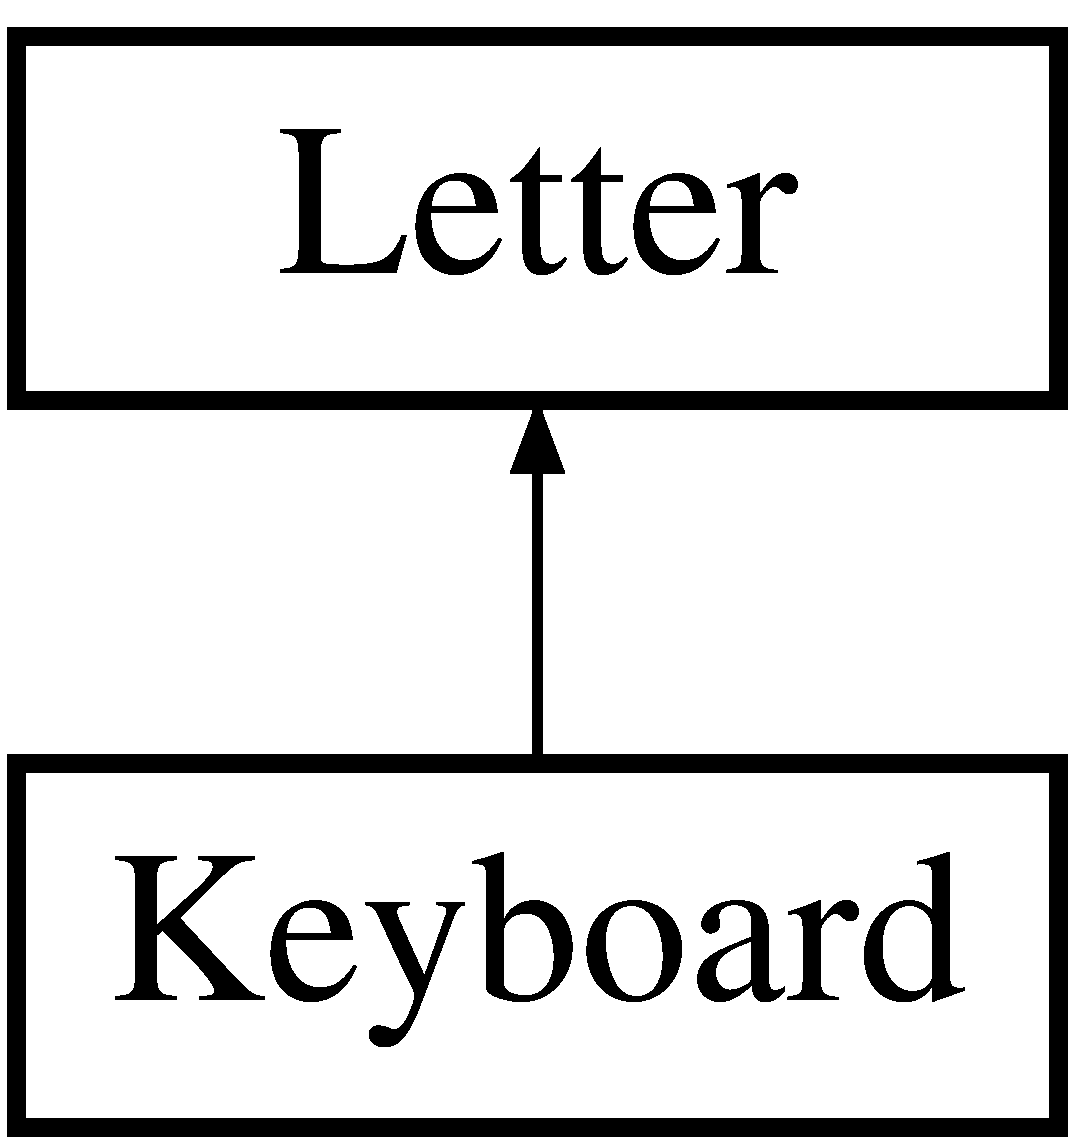
\includegraphics[height=2.000000cm]{class_keyboard}
\end{center}
\end{figure}
\subsection*{Public Member Functions}
\begin{DoxyCompactItemize}
\item 
\hypertarget{class_keyboard_ab709f4e952b99660d72624f0493016e4}{}\label{class_keyboard_ab709f4e952b99660d72624f0493016e4} 
void {\bfseries use} (int i)
\item 
\hypertarget{class_keyboard_a1857f3cb6f908638aa6296285fc15e9e}{}\label{class_keyboard_a1857f3cb6f908638aa6296285fc15e9e} 
bool {\bfseries is\+Used} (int i)
\item 
\hypertarget{class_keyboard_a4d7628f0662938e4f41cd49acc659224}{}\label{class_keyboard_a4d7628f0662938e4f41cd49acc659224} 
char {\bfseries get\+Char} (int i)
\item 
\hypertarget{class_keyboard_aed02d9f56fb12f4cec1129de092913d1}{}\label{class_keyboard_aed02d9f56fb12f4cec1129de092913d1} 
void {\bfseries display} () override
\item 
\hypertarget{class_keyboard_a5b4f3bd7c70e78197c806d1d81f499fe}{}\label{class_keyboard_a5b4f3bd7c70e78197c806d1d81f499fe} 
void {\bfseries set\+Arr} ()
\end{DoxyCompactItemize}
\subsection*{Public Attributes}
\begin{DoxyCompactItemize}
\item 
\hypertarget{class_keyboard_adf2f8d421d24de89f1e54fe7a17d2741}{}\label{class_keyboard_adf2f8d421d24de89f1e54fe7a17d2741} 
\hyperlink{class_letter}{Letter} $\ast$ {\bfseries arr}
\end{DoxyCompactItemize}
\subsection*{Additional Inherited Members}


The documentation for this class was generated from the following files\+:\begin{DoxyCompactItemize}
\item 
Keyboard.\+h\item 
Keyboard.\+cpp\end{DoxyCompactItemize}

\hypertarget{class_letter}{}\section{Letter Class Reference}
\label{class_letter}\index{Letter@{Letter}}
Inheritance diagram for Letter\+:\begin{figure}[H]
\begin{center}
\leavevmode
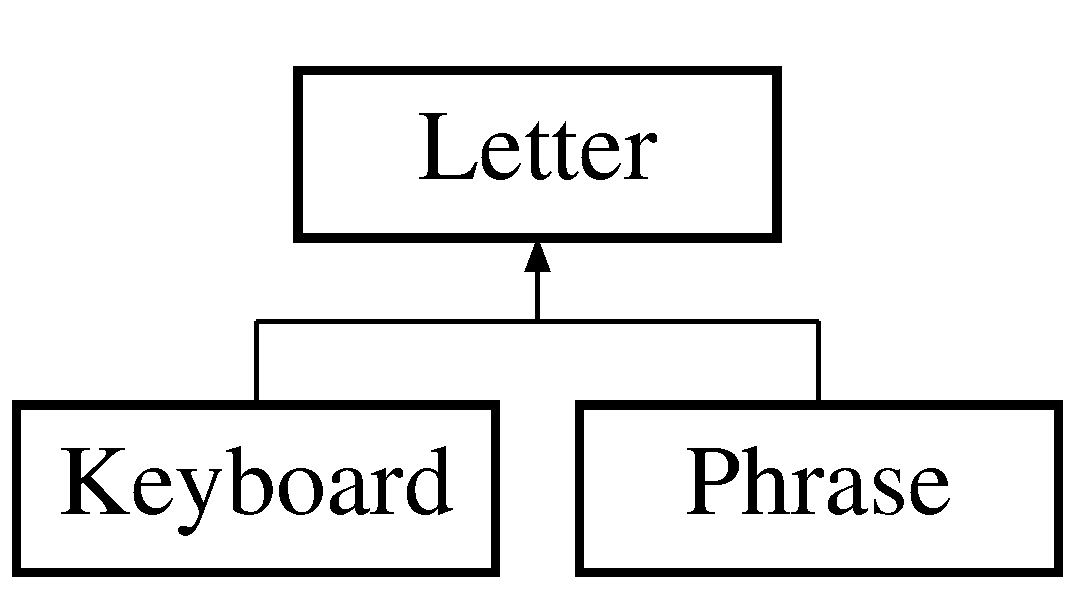
\includegraphics[height=2.000000cm]{class_letter}
\end{center}
\end{figure}
\subsection*{Public Member Functions}
\begin{DoxyCompactItemize}
\item 
\hypertarget{class_letter_a3bee19251225ca9f2f958191a5a7daba}{}\label{class_letter_a3bee19251225ca9f2f958191a5a7daba} 
{\bfseries Letter} (char)
\item 
\hypertarget{class_letter_ab4c06bc667637903013f93cc30fcde58}{}\label{class_letter_ab4c06bc667637903013f93cc30fcde58} 
void {\bfseries set\+Char} (char a)
\item 
\hypertarget{class_letter_a3de38802f3c236230882da7b83f930c4}{}\label{class_letter_a3de38802f3c236230882da7b83f930c4} 
void {\bfseries use} ()
\item 
\hypertarget{class_letter_a3b48f5b3d03e4a48d34d5a40c2af5190}{}\label{class_letter_a3b48f5b3d03e4a48d34d5a40c2af5190} 
char {\bfseries get\+Letter} ()
\item 
\hypertarget{class_letter_ae6ee6c11da6b6980f3860325ab5a9af1}{}\label{class_letter_ae6ee6c11da6b6980f3860325ab5a9af1} 
bool {\bfseries is\+Lt\+Used} ()
\item 
\hypertarget{class_letter_a5c54b5095ed21b6c68a7c8ef2d33b1a0}{}\label{class_letter_a5c54b5095ed21b6c68a7c8ef2d33b1a0} 
virtual void {\bfseries display} ()
\end{DoxyCompactItemize}
\subsection*{Static Public Member Functions}
\begin{DoxyCompactItemize}
\item 
\hypertarget{class_letter_a99f0b819c673c8cd9891934ba7ca6121}{}\label{class_letter_a99f0b819c673c8cd9891934ba7ca6121} 
static int {\bfseries call\+Use} ()
\end{DoxyCompactItemize}
\subsection*{Protected Attributes}
\begin{DoxyCompactItemize}
\item 
\hypertarget{class_letter_add29e231aa209f890a891ea202dbff4a}{}\label{class_letter_add29e231aa209f890a891ea202dbff4a} 
char {\bfseries letter}
\item 
\hypertarget{class_letter_ad1996ff2106ebfad001df34fd2484a0a}{}\label{class_letter_ad1996ff2106ebfad001df34fd2484a0a} 
bool {\bfseries is\+Used}
\end{DoxyCompactItemize}
\subsection*{Static Protected Attributes}
\begin{DoxyCompactItemize}
\item 
\hypertarget{class_letter_a8cb651b8860e525ee90780e5915d9955}{}\label{class_letter_a8cb651b8860e525ee90780e5915d9955} 
static int {\bfseries calls} =0
\end{DoxyCompactItemize}


The documentation for this class was generated from the following files\+:\begin{DoxyCompactItemize}
\item 
J\+B\+\_\+\+C\+S\+C17a/\+Project/\+Wheel\+Of\+Fortune\+\_\+v7/Letter.\+h\item 
J\+B\+\_\+\+C\+S\+C17a/\+Project/\+Wheel\+Of\+Fortune\+\_\+v7/Letter.\+cpp\end{DoxyCompactItemize}

\hypertarget{class_phrase}{}\section{Phrase Class Reference}
\label{class_phrase}\index{Phrase@{Phrase}}
Inheritance diagram for Phrase\+:\begin{figure}[H]
\begin{center}
\leavevmode
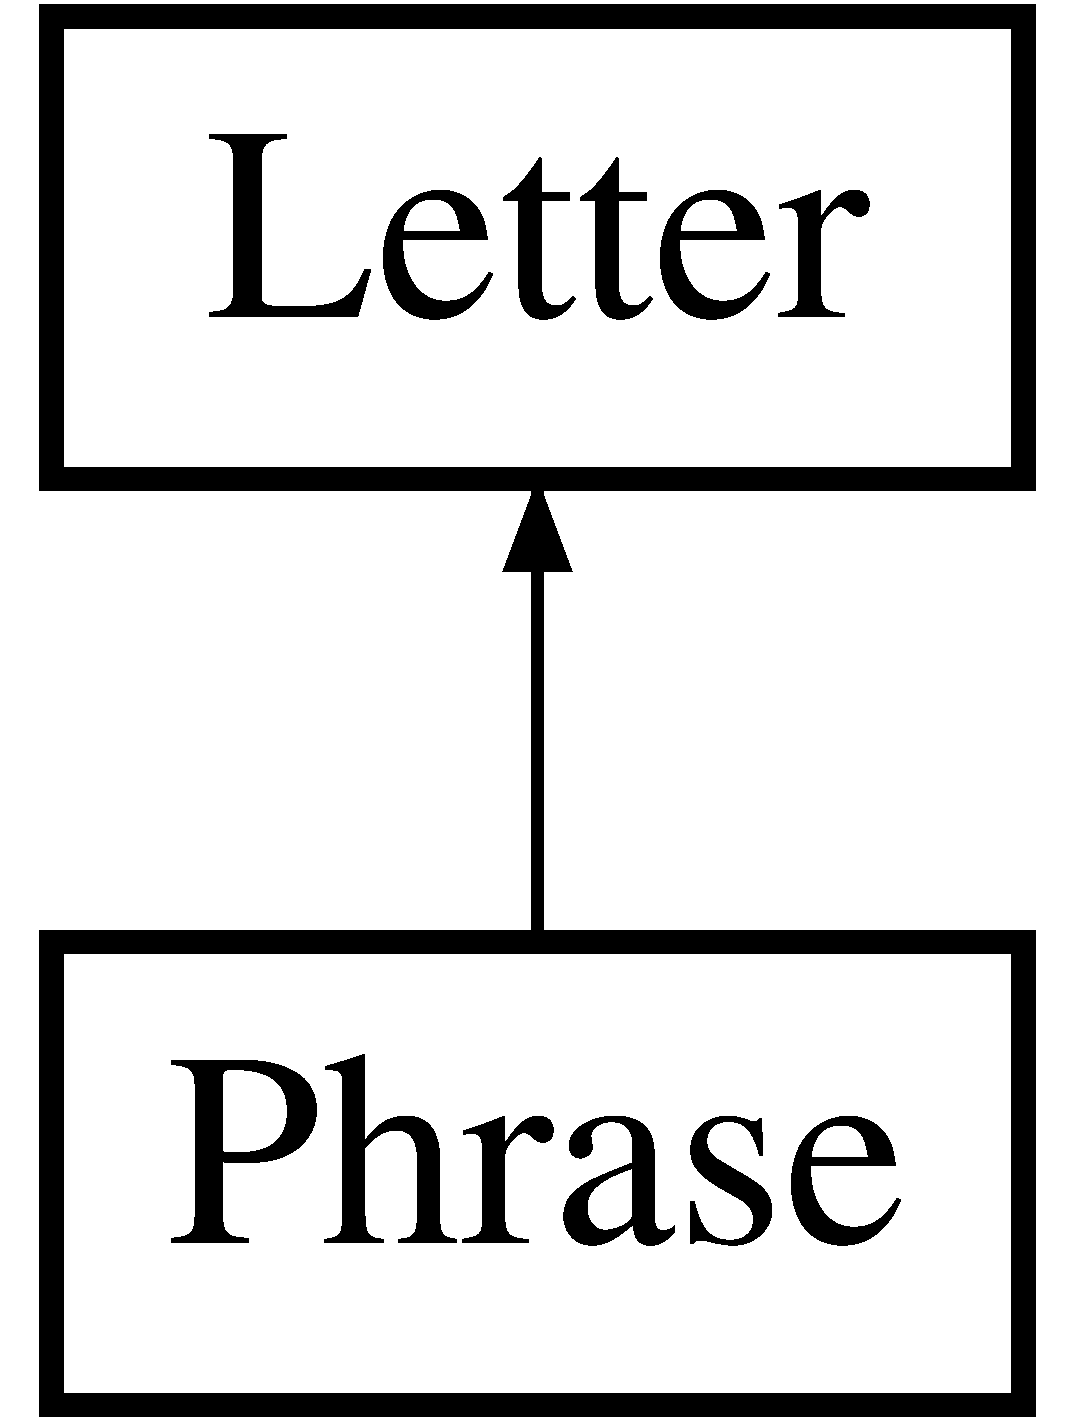
\includegraphics[height=2.000000cm]{class_phrase}
\end{center}
\end{figure}
\subsection*{Public Member Functions}
\begin{DoxyCompactItemize}
\item 
\hypertarget{class_phrase_aad8eb600a46aa1ffc25d7e0cb832f39b}{}\label{class_phrase_aad8eb600a46aa1ffc25d7e0cb832f39b} 
void {\bfseries use} (int i)
\item 
\hypertarget{class_phrase_a8144c049dc65c586127262d367545c20}{}\label{class_phrase_a8144c049dc65c586127262d367545c20} 
int {\bfseries get\+Size} ()
\item 
\hypertarget{class_phrase_a37e468274bd22c24e4cd1b76da578a72}{}\label{class_phrase_a37e468274bd22c24e4cd1b76da578a72} 
char {\bfseries get\+Letter} (int)
\item 
\hypertarget{class_phrase_a6144cc3eeb1f836b17e3d5f27d8eeec4}{}\label{class_phrase_a6144cc3eeb1f836b17e3d5f27d8eeec4} 
bool {\bfseries get\+Used} (int)
\item 
\hypertarget{class_phrase_ac673baf27de8946062e8f7846d2eb35c}{}\label{class_phrase_ac673baf27de8946062e8f7846d2eb35c} 
void {\bfseries set\+Arr} (unsigned int, string)
\item 
\hypertarget{class_phrase_a5913994bf6d88d27010ea27c7ed5a9ff}{}\label{class_phrase_a5913994bf6d88d27010ea27c7ed5a9ff} 
void {\bfseries display} () override
\end{DoxyCompactItemize}
\subsection*{Additional Inherited Members}


The documentation for this class was generated from the following files\+:\begin{DoxyCompactItemize}
\item 
Phrase.\+h\item 
Phrase.\+cpp\end{DoxyCompactItemize}

\hypertarget{class_play}{}\section{Play Class Reference}
\label{class_play}\index{Play@{Play}}
\subsection*{Public Member Functions}
\begin{DoxyCompactItemize}
\item 
\hypertarget{class_play_a0b4498cdd62a8eebeb10234185e3409d}{}\label{class_play_a0b4498cdd62a8eebeb10234185e3409d} 
void {\bfseries play} (\hyperlink{class_game}{Game} $\ast$)
\item 
\hypertarget{class_play_a7393a0885cbb8d087d657eb430ae5949}{}\label{class_play_a7393a0885cbb8d087d657eb430ae5949} 
void {\bfseries end} (\hyperlink{class_game}{Game} $\ast$)
\item 
\hypertarget{class_play_ae24e22ff4f1c68ae38f987ab066af7bb}{}\label{class_play_ae24e22ff4f1c68ae38f987ab066af7bb} 
void {\bfseries spin} (\hyperlink{class_game}{Game} $\ast$)
\item 
\hypertarget{class_play_ae353cd9ddff43a03f5c7d1f29d99dd57}{}\label{class_play_ae353cd9ddff43a03f5c7d1f29d99dd57} 
void {\bfseries buy} (\hyperlink{class_game}{Game} $\ast$)
\item 
\hypertarget{class_play_a56e8356e639427c516bc83761818ca77}{}\label{class_play_a56e8356e639427c516bc83761818ca77} 
void {\bfseries guess} (\hyperlink{class_game}{Game} $\ast$)
\item 
\hypertarget{class_play_ae9d057ab4c97d7d676ea365ee910cde3}{}\label{class_play_ae9d057ab4c97d7d676ea365ee910cde3} 
void {\bfseries display} ()
\item 
\hypertarget{class_play_a6af79117e524b01d8aa77ad6b3a75c6d}{}\label{class_play_a6af79117e524b01d8aa77ad6b3a75c6d} 
void {\bfseries menu} (\hyperlink{class_game}{Game} $\ast$)
\item 
\hypertarget{class_play_ac8244da334ad843bffa229010b909ad3}{}\label{class_play_ac8244da334ad843bffa229010b909ad3} 
bool {\bfseries get\+Win} ()
\item 
\hypertarget{class_play_a996f01a55184ef4f63c9e54b742d18ad}{}\label{class_play_a996f01a55184ef4f63c9e54b742d18ad} 
int {\bfseries get\+Money} (\hyperlink{class_game}{Game} $\ast$a)
\end{DoxyCompactItemize}


The documentation for this class was generated from the following files\+:\begin{DoxyCompactItemize}
\item 
J\+B\+\_\+\+C\+S\+C17a/\+Project/\+Wheel\+Of\+Fortune\+\_\+v7/Play.\+h\item 
J\+B\+\_\+\+C\+S\+C17a/\+Project/\+Wheel\+Of\+Fortune\+\_\+v7/Play.\+cpp\end{DoxyCompactItemize}

\hypertarget{struct_player}{}\section{Player Struct Reference}
\label{struct_player}\index{Player@{Player}}
\subsection*{Public Member Functions}
\begin{DoxyCompactItemize}
\item 
\hypertarget{struct_player_ac13db53be14f078b1c7e9e4750f21ac6}{}\label{struct_player_ac13db53be14f078b1c7e9e4750f21ac6} 
void {\bfseries operator+} (int n)
\item 
\hypertarget{struct_player_add3e9da9c3925ecab8ccd15c1d14ef52}{}\label{struct_player_add3e9da9c3925ecab8ccd15c1d14ef52} 
void {\bfseries operator-\/} (int n)
\end{DoxyCompactItemize}
\subsection*{Public Attributes}
\begin{DoxyCompactItemize}
\item 
\hypertarget{struct_player_acf0355128a99ee20ad9931b760fb2de1}{}\label{struct_player_acf0355128a99ee20ad9931b760fb2de1} 
string {\bfseries name}
\item 
\hypertarget{struct_player_a9545beef70350d5c3b3a5719a890dd2f}{}\label{struct_player_a9545beef70350d5c3b3a5719a890dd2f} 
int {\bfseries money}
\item 
\hypertarget{struct_player_a38a6dafe988a768a435cc0a9fde38e46}{}\label{struct_player_a38a6dafe988a768a435cc0a9fde38e46} 
unsigned int {\bfseries score}
\end{DoxyCompactItemize}


The documentation for this struct was generated from the following file\+:\begin{DoxyCompactItemize}
\item 
Player.\+h\end{DoxyCompactItemize}

%--- End generated contents ---

% Index
\backmatter
\newpage
\phantomsection
\clearemptydoublepage
\addcontentsline{toc}{chapter}{Index}
\printindex

\end{document}
